%%%%%%%%%%%%%%%%%%%%%%%%%%%%%%%%%%%%%%%%%
% Barbara Liskov Presentation
% LaTeX Template
% 23/11/2020
% 
%%%%%%%%%%%%%%%%%%%%%%%%%%%%%%%%%%%%%%%%%

%------------------------------------------------------------------
%	PACKAGES AND THEMES
%------------------------------------------------------------------

\documentclass{beamer}

\mode<presentation> {

\usetheme{Madrid}

}
\hypersetup{
    colorlinks=true,
    linkcolor=blue,
    filecolor=magenta,      
    urlcolor=cyan,
}
\usepackage{graphicx} 
\usepackage{booktabs} 
\usepackage{hyperref} 
\usepackage{listings}

\usepackage{xcolor}

\definecolor{codegreen}{rgb}{0,0.6,0}
\definecolor{codegray}{rgb}{0.5,0.5,0.5}
\definecolor{codepurple}{rgb}{0.58,0,0.82}
\definecolor{backcolour}{rgb}{0.95,0.95,0.92}



\lstdefinestyle{mystyle}{
    backgroundcolor=\color{backcolour},   
    commentstyle=\color{codegreen},
    keywordstyle=\color{magenta},
    numberstyle=\tiny\color{codegray},
    stringstyle=\color{codepurple},
    basicstyle=\ttfamily\footnotesize,
    breakatwhitespace=false,         
    breaklines=true,                 
    captionpos=b,                    
    keepspaces=true,                 
    numbers=left,                    
    numbersep=5pt,                  
    showspaces=false,                
    showstringspaces=false,
    showtabs=false,                  
    tabsize=2
}

\lstset{style=mystyle}

%-----------------------------------------------------------------
%	TITLE PAGE
%-----------------------------------------------------------------

\title[Research Methods]{Barbara Liskov}
\author{Group N}
\institute[GMIT]
{
\textit{Grace Keane} \\\textit{Shirin Nagle} \\ 
\medskip
}
\date{}

\begin{document}

\begin{frame}
\titlepage % Print the title page as the first slide
\end{frame}

%------------------------------------------------------------------
%	BRIEF DESCRIPTION
%------------------------------------------------------------------

\begin{frame}
\frametitle{Brief Description} 

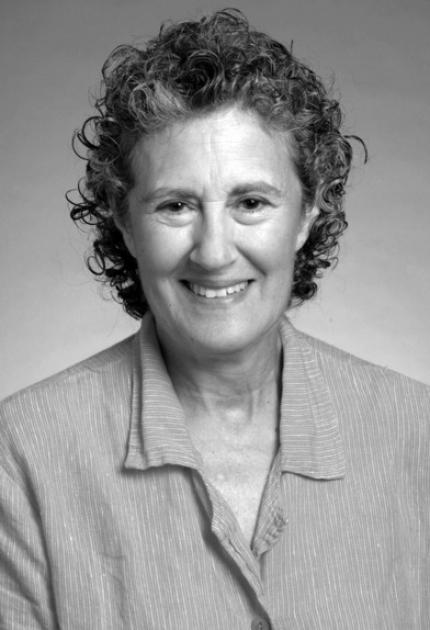
\includegraphics[scale=0.4]{Barbara Liskov}
\centering

\end{frame}


%----------------------------------------------------------------
%	PRESENTATION SLIDES
%----------------------------------------------------------------

\begin{frame}
\frametitle{Important Details}
\begin{itemize}
\item Computer Scientist
\item Born: November 7th, 1939, California
\item One of the first women in the USA to be awarded a PhD in Computer Science
\item She is one of the world's leading authorities on computer language and system design
\item She won numerous awards as well as the Turing award in 2009
\item Since 1966, 70 computer scientists have won the Turing Award. Only 3 have been women. Therefore this is an amazing achievement
\item Created the Liskov's substitution principle
\end{itemize}
\end{frame}

%------------------------------------------------
\begin{frame}
\frametitle{Barbara Liskov Timeline}

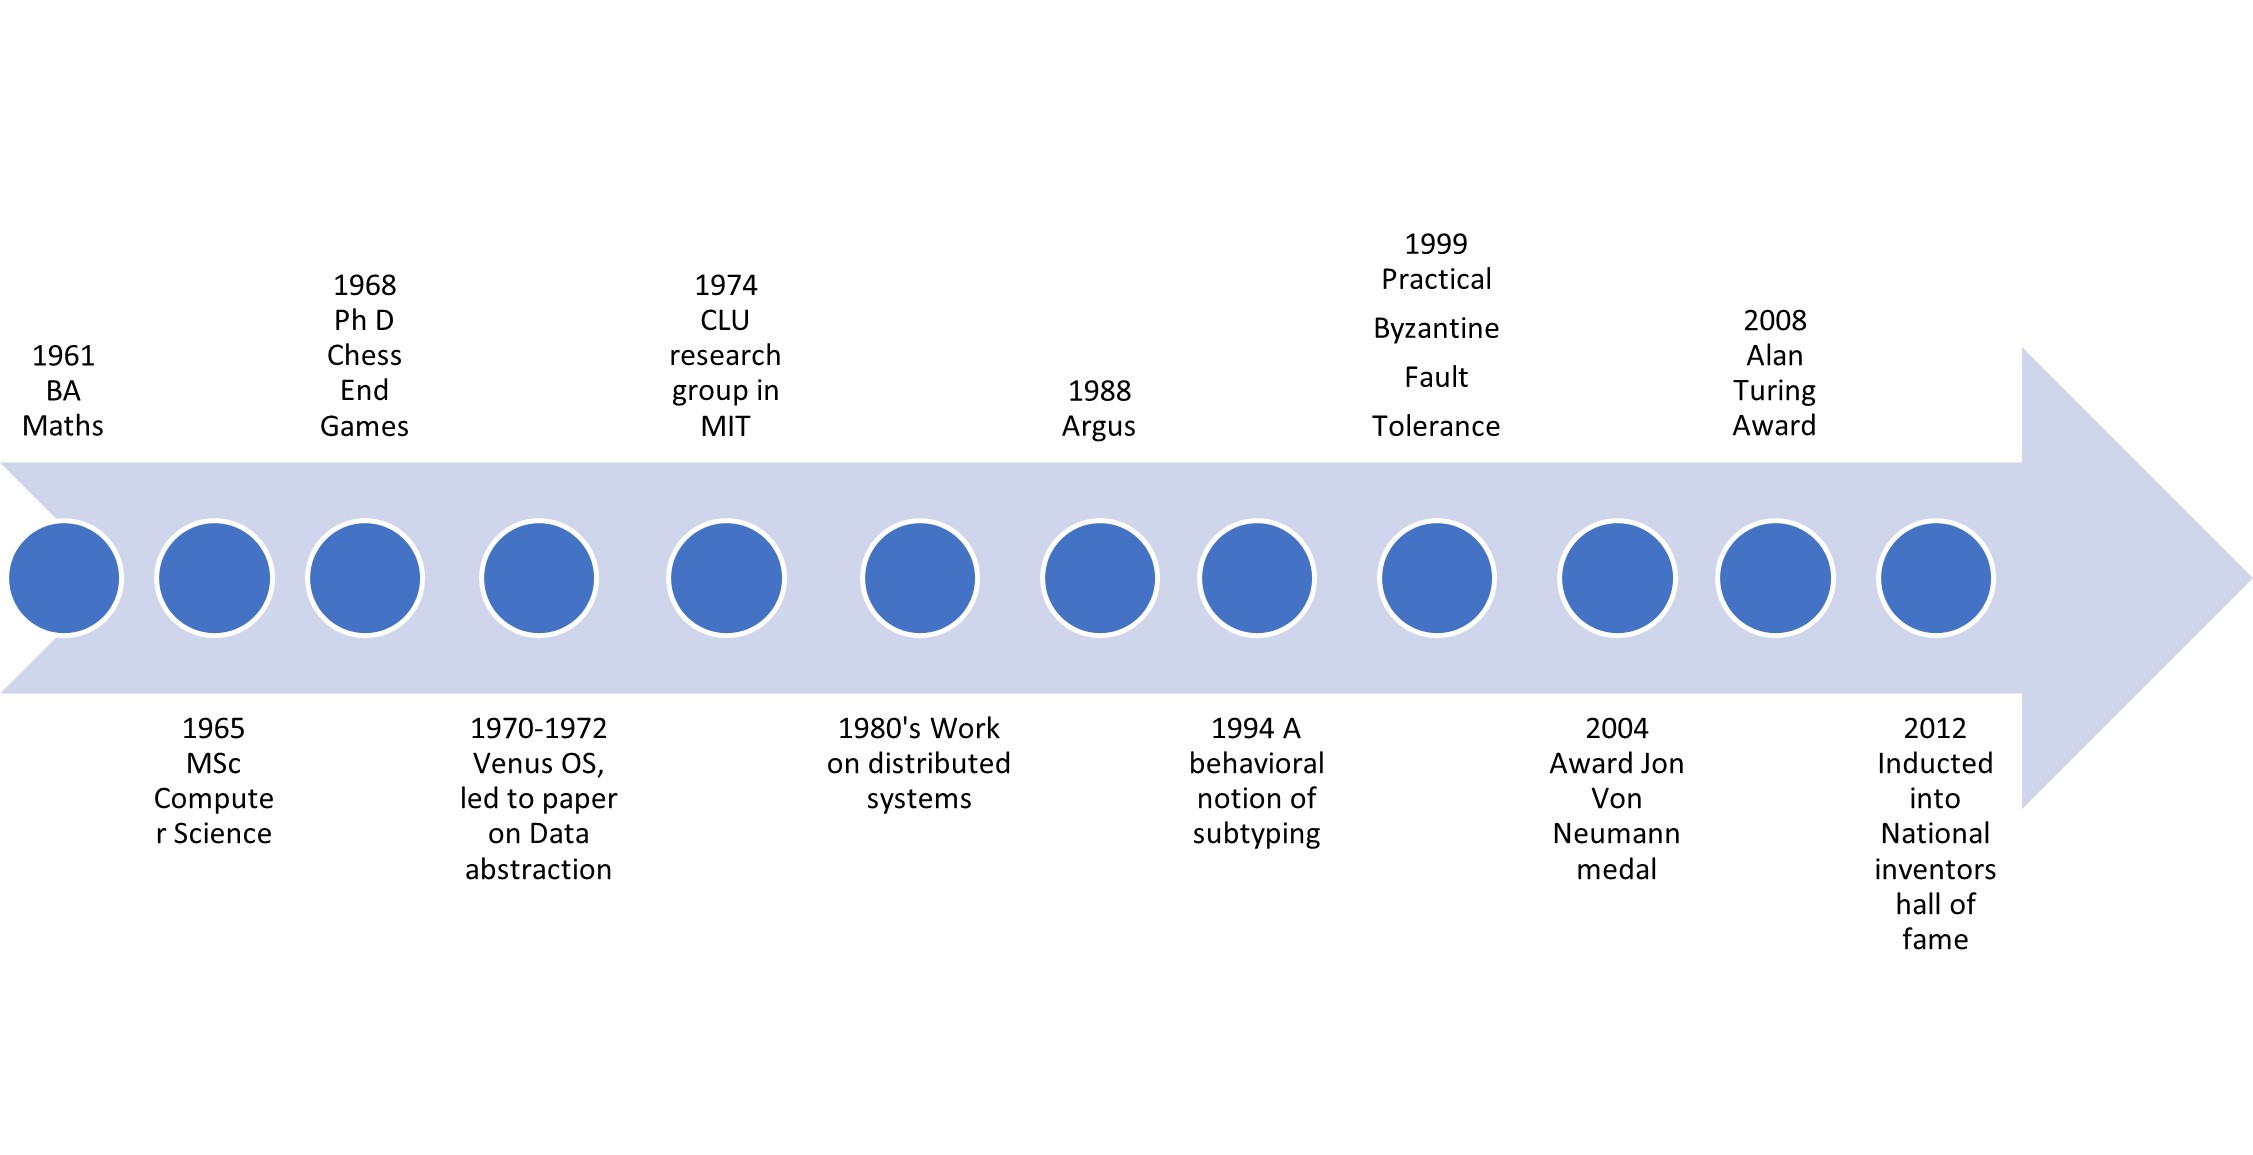
\includegraphics[scale=0.7]{timeline.jpg}

    
\end{frame}
%------------------------------------------------
\begin{frame}
\frametitle{Turing Award Citation}
Barbara Liskov was awarded the Alan Turing award in 2008 for  contributions "of lasting and major technical importance to the computer field". 

\vspace{5mm} %5mm vertical space

Award for contributions to practical and theoretical foundations of programming language and system design, especially related to data abstraction, fault tolerance, and distributed computing. 

\vspace{5mm}

\end{frame}

%------------------------------------------------

\begin{frame}
\frametitle{Selected work}
\begin{itemize}
\item Data Abstraction.
\item CLU Programming Language.
\item Liskov Substitution.
\item Distributed Systems.
\item Practical Byzantine Fault Tolerance.
\end{itemize}
\end{frame}
%------------------------------------------------


%------------------------------------------------
\begin{frame}
\frametitle{Data Abstraction}
Because  systems  of  any  size  can  always  be  expected  to  be  subject  to  changes  in  requirements,  the  project  goal  is  to  produce  not  only  reliable  software,  but  readable  software  which  is relatively  easy  to  modify  and  maintain[5].

\vspace{5mm}

What we desire from an abstraction is a mechanism which permits the expression of relevant details and the suppression of irrelevant details. In the case of programming, the use which may be made of an abstraction is relevant; the way in which the abstraction is implemented is irrelevant[6]. 

\vspace{5mm}

This work resulted in CLU a programming language which is a predecessor to many OOP languages.

\vspace{5mm}

Her contributions have influenced advanced system developments and set a standard for clarity and usefulness

\end{frame}
%------------------------------------------------

%------------------------------------------------
\begin{frame}
\frametitle{CLU Programming Language}

At MIT she led the design and implementation of the CLU programming language, which emphasized the notions of modular programming, data abstraction, and polymorphism. These concepts are a foundation of object-oriented programming used in modern computer languages such as Java and C\#.

\vspace{5mm}

CLU introduced many features that are used widely now, and is seen as a step in the development of object-oriented programming and was also notable for its use of classes with constructors and methods, but without inheritance [1].

\end{frame}
%------------------------------------------------
\begin{frame}{Cluster template in CLU}

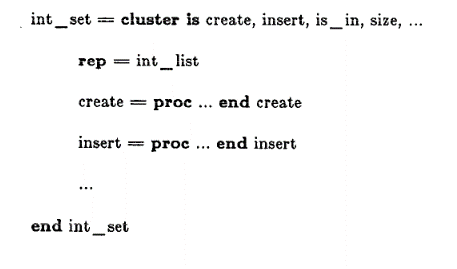
\includegraphics{cluster.png}
    
\end{frame}


%------------------------------------------------
\begin{frame}
\frametitle{Barbara Liskov's definition}

Developed a new notion of sub typing now known as the Liskov Substitution principle.

\vspace{5mm} %5mm vertical space

At a high level, the LSP states that in an object-oriented program, if we substitute a superclass object reference with an object of any of its subclasses, the program should not break [2].\\

\vspace{5 mm}

"If for each object o1 of type S there is an object o2 of type T such that for all programs P defined in terms of T, the behavior of P is unchanged when o1 is substituted for o2 then S is a subtype of T"


\end{frame}



%------------------------------------------------

\vspace{5mm}

% Putting code on screen & formatted nicely
\begin{lstlisting}[language=Java]
[3]
// Animal super class 
public static class Animal {
  public String favoriteFood;
  public Animal(String favoriteFood) {
    this.favoriteFood = favoriteFood;
  }
}
// Subclass
public static class Dog extends Animal {
  public Dog(String favoriteFood) {
    super(favoriteFood);
  }
}

// Subclass
public static class Cat extends Animal {
  public Cat(String favoriteFood) {
    super(favoriteFood);
  }
}
\end{lstlisting}

\vspace{5mm}

%------------------------------------------------

%------------------------------------------------

\vspace{5mm}
[3]
% Putting code on screen & formatted nicely
\begin{lstlisting}[language=Java]
// Method to give treats
public static void GiveTreatTo(Animal animal) {
  String msg = "You fed the " + animal.getClass().getSimpleName() + " some "  + animal.favoriteFood;
  System.out.println(msg);
}

// Assigning treats to animals
// Do not have to create a new method per animal because of the LSP principle
public static void main(String[] args) {
  Dog rover = new Dog("bacon");
  Cat bingo = new Cat("fish");

  GiveTreatTo(rover);
  GiveTreatTo(bingo);
}
Command prompt output:

You gave the Dog some bacon
You gave the Cat some fish
\end{lstlisting}

%------------------------------------------------

\begin{frame}
\frametitle{SOLID} 

\includegraphics[scale=0.8]{SOLID}
\centering


\end{frame}

%------------------------------------------------

\begin{frame}
\frametitle{Principle naming}
She did not name the Liskov Substitution Principle. Apparently, she received an email in the 90’s by somebody asking her whether he got her principle right, surprising her. She had not known that the principle had borne her name for years in the community.
\end{frame}

%------------------------------------------------
\begin{frame}{Distributed Systems}
In the 1980’s remote file systems came into existence. Worked on an algorithm that handled benign failures or crash failures.
 Designed a replication technique with Brian Oki[7].
 
 \vspace{2mm}
 
 One of the potential benefits of distributed systems is their use in providing highly-available services, that is, services that are likely to be up and accessible when needed. Availability is essential to many computer-based services; for example, in airline reservation systems the failure of a single computer can prevent ticket sales for a considerable time, causing a loss of revenue and passenger goodwill. Availability is achieved through replication. By having more than one copy of important information, the service continues to be usable even when some copies are inaccessible, for example, because of a crash of the computer where a copy was stored[7].


    
\end{frame}
%------------------------------------------------
%------------------------------------------------
\begin{frame}{Practical Byzantine Fault Tolerance}
In the 1990's came up with a new replication algorithm that  is able to tolerate Byzantine faults with Miguel Castro[8].

\vspace{2mm}

pBFT consensus rounds are called views and are broken into 4 phases:

    \vspace{3mm}
    
   1. A client sends a request to the leader node to invoke a service operation.
   \newline
   
   2. The leading node broadcasts the request to the backup nodes.
   \newline
  
    3.The nodes execute the request, then send a reply to the client.
    \newline
    
   4. The client awaits f+1 replies from different nodes with the same result, where f represents the maximum number of potentially faulty nodes[9].
   
   \vspace{1mm}

\end{frame}
%------------------------------------------------


\begin{frame}{Conclusion}
\begin{itemize}
\item At 81, Barbara Liskov is still active today contributing to and writing many papers as recently as this year.
\item Subsequent work has mainly been in the area of distributed systems. 
\item Her research has covered many aspects of OS and computation \begin{itemize}
    \item work on object-oriented database systems
    \item  garbage collection
    \item caching, persistence, recovery, 
    \item security, decentralized information flow
    \item modular upgrading of distributed systems, geographic routing
    \item fault tolerance and practical Byzantine fault tolerance
\end{itemize}  
\item Many of these, deal with situations where a complex system fails in arbitrary ways. 
\item Liskov developed methods to allow correct operation even when some components are unreliable.
 

\end{itemize}
\end{frame}



%------------------------------------------------

\begin{frame}
\Huge{\centerline{The End}}
\end{frame}

%-----------------------------------------------------------------
\begin{frame}{References}

[1] {CLU (programming language)} https://en.wikipedia.org/wiki/CLU_(programming_language)

[2] {The Liskov Substitution Principle Explained} https://reflectoring.io/lsp-explained/

\vspace{1mm}

[3] {Liskov Substitution Principle in 3 Minutes}
https://dev.to/erikwhiting88/liskov-substitution-principle-in-3-minutes-2dc6

\vspace{1mm}

[4] {SOLID Principle in Programming: Understand With Real Life Examples}

https://www.geeksforgeeks.org/solid-principle-in-programming-understand-with-real-life-examples/#:~:text=Liskov's%20Substitution%20Principle%3A%20The%20principle,their%20base%20or%20parent%20classes%E2%80%9C.&text=So%20we%20can%20say%20that,rectangle%20class%20into%20square%20class.

\end{frame}

%-----------------------------------------------------------------
\begin{frame}{References}

[5] {A  design  methodology  for  reliable  software   systems, Barbara Liskov, 1972} https://ckrybus.com/static/papers/liskov1972.pdf 

\vspace{1mm}

[6] {Programming With Abstract Data Types - B.Liskov 1974}
http://web.cs.iastate.edu/~hridesh/teaching/362/07/01/papers/p50-liskov.pdf

\vspace{1mm}

[7] {Viewstamped Replication: A New Primary Copy Method to Support Highly-Available Distributed Systems B. Liskov, B.Oki 1988}
http://pmg.csail.mit.edu/papers/vr.pdf

\vspace{1mm}

[8] {PracticalByzantineFaultTolerance M.Castro, B. Liskov 1999} http://pmg.csail.mit.edu/papers/osdi99.pdf

\vspace{1mm}

[9] https://crushcrypto.com/what-is-practical-byzantine-fault-tolerance/


\end{frame}


%-----------------------------------------------------------------


\begin{frame}
\frametitle{Clickable References}
\begin{itemize}
\item \href{https://amturing.acm.org/award_winners/liskov_1108679.cfm}{ A.M. Turing; Barbara Liskov;} 

\item \href {https://dl.acm.org/doi/abs/10.1145/155360.155367}{A history of CLU Barbara Liskov (1992)}

\item \href{https://dblp.uni-trier.de/pid/l/BarbaraLiskov.html}{Barbara Liskov Index of publications}

\item \href{http://www.pmg.csail.mit.edu/~liskov/newcv-09.pdf}{Barbara Liskov CV}

\item \href{http://www.pmg.csail.mit.edu/~liskov/}{Barbara Liskov home page}

\item \href{https://citeseerx.ist.psu.edu/viewdoc/download?doi=10.1.1.46.9499&rep=rep1&type=pdf}{A History of CLU, Barbara Liskov 1992}
\end{itemize}
\end{frame}

%-----------------------------------------------

\begin{frame}
\frametitle{GitHub link}

Organization used to manage our LaTeX presentation progression

\vspace{5mm}


\href{https://github.com/Research-Methods-Presentation}{GitHub organisation link} 

\end{frame}

%-----------------------------------------------

\begin{frame}
\Huge{\centerline{Questions?}}
\end{frame}

%-----------------------------------------------


\end{document} 